\beginsong{Bürgerlied}[
    mel={Prinz Eugen, der edle Ritter}, 
    meljahr={ca. 1845},
    txt={Adalbert Harnisch}, 
    txtjahr={1845}
    tonspur={432}, 
    buedel={229}, 
    index={Ob wir rote, gelbe Kragen},
]

\beginverse 
\endverse
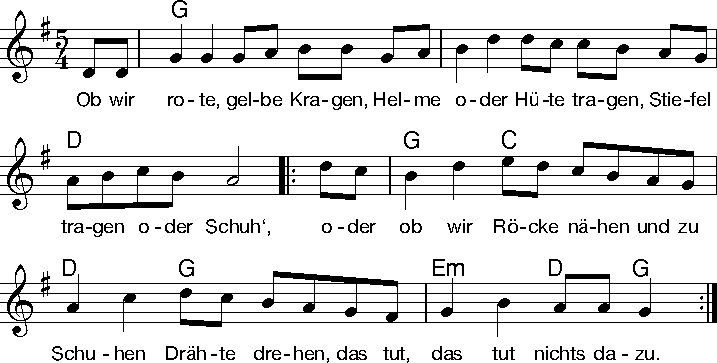
\includegraphics[draft=false, width=1\textwidth]{Noten/Lied011a.pdf}

\beginverse
Ob wir \[G]können präsidieren
oder müssen Akten schmieren ohne \[D]Rast und ohne Ruh,
ob wir \[G]just Coll\[C]egia lesen 
oder \[D]aber \[G]binden Besen, das tut, \[Em]das tut \[D]nichts da\[G]zu.
\endverse

\beginverse
Ob wir ^stolz zu Rosse reiten, 
oder ob zu Fuß wir schreiten barfuß ^unser'm Ziele zu,
ob uns ^Kreuze ^vorne schmücken 
oder ^Kreuze ^hinten drücken, das tut, ^das tut ^nichts da^zu.
\endverse

\beginverse
Aber ^ob wir Neues bauen 
oder Altes nur verdauen, wie das ^Gras verdaut die Kuh,
ob wir ^in der ^Welt was schaffen 
oder ^nur die ^Welt begaffen, das tut, ^das tut ^was da^zu.
\endverse

\beginverse
Ob wir ^rüstig und geschäftig, 
wo es gilt zu wirken kräftig, immer ^tapfer greifen zu,
oder ^ob wir ^schläfrig denken: 
„Gott wird's ^wohl im ^Schlafe lenken“, das tut, ^das tut ^was da^zu.
\endverse

\beginverse
Ob im ^Kopfe etwas Grütze 
und im Herzen Licht und Hitze, dass es ^brennt in einem Nu,
oder ^ob wir ^hinter Mauern 
immer ^stets im ^Dunkeln kauern: Das tut, ^das tut ^was da^zu.
\endverse

\beginverse
D'rum, ihr ^Bürger, d'rum, 
ihr Brüder, alle eines Bundes Glieder, was auch ^jeder von uns tu'. 
Alle, ^die dies ^Lied gesungen, 
so die ^Alten, ^wie die Jungen: Tun wir, ^tun wir ^was da^zu!
\endverse

\endsong

\beginscripture{}
Das Lied wurde im Mai 1845 für den "Bürgerverein" der Stadt Elging geschrieben, um die Vision eines liberal gesinnten Bürgertums eines einigen deutschen Staates auszudrücken. Das Lied wurde während der Märzrevolution 1848/1849 auf Flugblättern verteilt. Nach der Revolution diente das Lied der neuen Arbeiterbewegung zum Ausdruck ihrer Forderung nach gesellschaftlicher Veränderung.
\endscripture
